%* 
%* ------------------------------------------------------------------
%* AN02_AutoDispatcher.tex - Application Note 2: Auto Dispatcher
%* Created by Robert Heller on Sun Oct 14 15:23:53 2012
%* ------------------------------------------------------------------
%* Modification History: $Log$
%* Modification History: Revision 1.1  2002/07/28 14:03:50  heller
%* Modification History: Add it copyright notice headers
%* Modification History:
%* ------------------------------------------------------------------
%* Contents:
%* ------------------------------------------------------------------
%*  
%*     Model RR System, Version 2
%*     Copyright (C) 1994,1995,2002-2012  Robert Heller D/B/A Deepwoods Software
%* 			51 Locke Hill Road
%* 			Wendell, MA 01379-9728
%* 
%*     This program is free software; you can redistribute it and/or modify
%*     it under the terms of the GNU General Public License as published by
%*     the Free Software Foundation; either version 2 of the License, or
%*     (at your option) any later version.
%* 
%*     This program is distributed in the hope that it will be useful,
%*     but WITHOUT ANY WARRANTY; without even the implied warranty of
%*     MERCHANTABILITY or FITNESS FOR A PARTICULAR PURPOSE.  See the
%*     GNU General Public License for more details.
%* 
%*     You should have received a copy of the GNU General Public License
%*     along with this program; if not, write to the Free Software
%*     Foundation, Inc., 675 Mass Ave, Cambridge, MA 02139, USA.
%* 
%*  
%* 

\chapter{Auto Dispatcher}
\label{chapt:AutoDispatcher}
\typeout{$Id$}

The software for this layout implements a simple automatic dispatching
system. Most of the time the trains are on a double track ``main line''
and require no dispatching, since each main line track segment is
operated in a single direction with only one train.  At the either end of the
layout is a segment of bi-directional single track.  Using 
Azatrax MRD2-U's the computer senses trains traveling through these
segments of bi-directional single track and uses Azatrax SR4-Us to
control the turnouts, signals, and the polarity of the power feed to the
segments of bi-directional single track, allowing only one train access
at a time.

Each segment of bi-directional single track, with associated turnouts
use two MRD2-U's (one for each logical direction) to sense trains.

\section{Dispatching Logic}

\begin{figure}[hbpt]
\begin{centering}
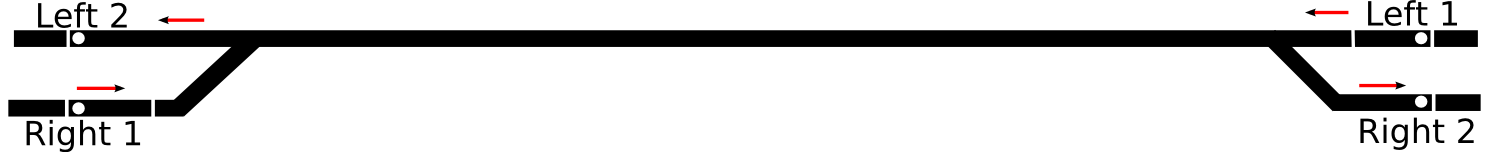
\includegraphics[width=5in]{singletrack-ink1.png}
\caption{Schematic of a bi-direction single track segment}
\label{fig:AutoDispatcher:singletrack-ink1}
\end{centering}
\end{figure}
A schematic track diagram of a bi-direction single track segment is
shown in Figure~\ref{fig:AutoDispatcher:singletrack-ink1}. There are
four sensor locations, shown as white dots and labeled \texttt{Left 1},
\texttt{Left 2}, \texttt{Right 1}, and \texttt{Right 2}.  These sensors
are connected to two MRD2-U, \texttt{Left} and \texttt{Right}. The
sensors are connected to the MRD2-U such that a given MRD2-U's ``sense
1'' is the entry and ``sense 2'' is the exit.  Each MRD2-U device thus
senses a train going in a specific direction through the single track
segment. There is a gap (eg with insulating rail joiners) between both
mainline tracks and the single track segment.  There is an additional
gap about the length of the engine past the entrance sensor.  This short
segment of track is powered via diodes from the rest of the single track
segment. The diodes enforce the correct direction of travel for the
entering train. The single track segment is considered occupied by a train
traveling from right to left if either of the left sensors are active
(the train is entering or leaving) or if the left sensor 1 latch is set
(the train is between sensors).  The  single track segment is
considered occupied by a train traveling from left to right if either
of the right sensors are active (the train is entering or leaving) or
if the right sensor 1 latch is set (the train is between sensors). 
When a train arrives at a sensor 1 position (either \texttt{Left 1} or
\texttt{Right 1}), the computer checks to see if the single track
segment is occupied by a train going in the opposite direction.



\section{The code, annotated.}


\begin{figure}[hbpt]\begin{centering}
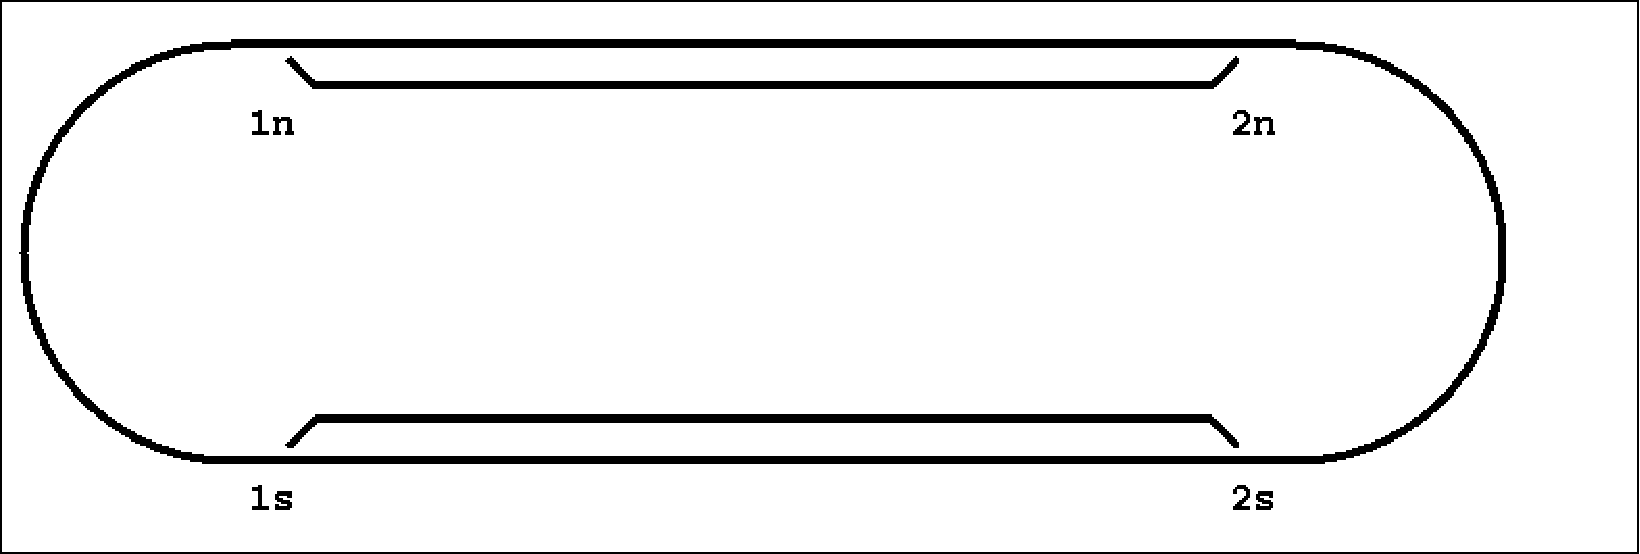
\includegraphics[width=5in]{AN02_schematic_rev.pdf}
\caption{Schematic of the layout}
\label{fig:an02log:AN02_schematic_rev}
\end{centering}
\end{figure}
Listing~\ref{lst:an02:dispatchinglogic} contains the user code section
of the dispatcher program for this layout. The displayed schematic of
the layout is shown in Figure~\ref{fig:an02log:AN02_schematic_rev}.

The code starts with a procedure named \texttt{CurveOccupancy}, starting
at line 268 of the source file (\texttt{AN02.tcl}). This procedure is
used by the single track curved sections at the east and west ends of
the layout to check for occupancy. It uses both MRD2-U units to test for
either a clockwise or counter-clockwise train occupying the curved
section (including the turnouts at the ends).

The next section, starting at line 314, defines a \texttt{SNIT} type to
handle the logic for occupancy checking for the four straight sections.
Four instances of this type are created, one for each of the straight
sections, starting at line 431.

Starting at line 446 is a pair of blocks of code to initialize the two
SR4 devices to a known powered up state.

At line 460 the main loop starts. The main loop starts by reading in the
state data of the six Azatrax devices.  This is done at lines 463--473.
Then all of the trackwork is ``invoked'', which runs the occupancy
scripts for each piece of trackwork and thus determines whether or not
the various blocks are occupied.  This is done at lines 475--492.

Next come 4 blocks of code, starting at line 494 that implement the
dispatcher logic, which is to check for a train arriving at an entry
detector and then testing to see if there is an opposing movement in
the single track block.  If the block is clear, the turnout is thrown
in favor of the entering train and the power reversing relay is set or
unset to also favor the entering train. There is a block of code for
each entrance sensor.  The four blocks of code are at lines 507--523
(West end clockwise block), 525--541 (West end counter-clockwise
block), 546--562 (East end clockwise block), and 564--580 (East end
counter-clockwise block).

At the bottom of the main loop is a call to the \texttt{update}, which
causes the GUI to update to reflect the state of the layout.

\lstinputlisting[caption={Dispatching logic, implemented in Tcl \texttt{AN02.tcl}},
		 label={lst:an02:dispatchinglogic},
		 firstline=268]{AN02.tcl}

